\documentclass{beamer}

\usefonttheme{professionalfonts} % using non standard fonts for beamer
\usefonttheme{serif} % default family is serif

\usepackage{hyperref}

%\usepackage{minted}

\usepackage{animate}

\usepackage{graphicx}

\def\Put(#1,#2)#3{\leavevmode\makebox(0,0){\put(#1,#2){#3}}}

\usepackage{color}

\usepackage{tikz}

\usepackage{amssymb}

\usepackage{enumerate}


\newcommand\blfootnote[1]{%

  \begingroup

  \renewcommand\thefootnote{}\footnote{#1}%

  \addtocounter{footnote}{-1}%

  \endgroup

}

\makeatletter

%%%%%%%%%%%%%%%%%%%%%%%%%%%%%% Textclass specific LaTeX commands.

 % this default might be overridden by plain title style

 \newcommand\makebeamertitle{\frame{\maketitle}}%

 % (ERT) argument for the TOC

 \AtBeginDocument{%

   \let\origtableofcontents=\tableofcontents

   \def\tableofcontents{\@ifnextchar[{\origtableofcontents}{\gobbletableofcontents}}

   \def\gobbletableofcontents#1{\origtableofcontents}

 }

%%%%%%%%%%%%%%%%%%%%%%%%%%%%%% User specified LaTeX commands.

\usetheme{Malmoe}

% or ...

\useoutertheme{infolines}

\addtobeamertemplate{headline}{}{\vskip2pt}



\setbeamercovered{transparent}

% or whatever (possibly just delete it)

\makeatother

\begin{document}
\title[DCEL report]{Parallel DCEL Construction Report}
\author[AC]{Andres Calderon}
\institute[Summer'19]{University of California, Riverside}
\makebeamertitle
\newif\iflattersubsect

\AtBeginSection[] {
    \begin{frame}<beamer>
    \frametitle{Outline} 
    \tableofcontents[currentsection]  
    \end{frame}
    \lattersubsectfalse
}

\AtBeginSubsection[] {
    \begin{frame}<beamer>
    \frametitle{Outline} 
    \tableofcontents[currentsubsection]  
    \end{frame}
}

\begin{frame}{DCEL construction}
    \centering 
    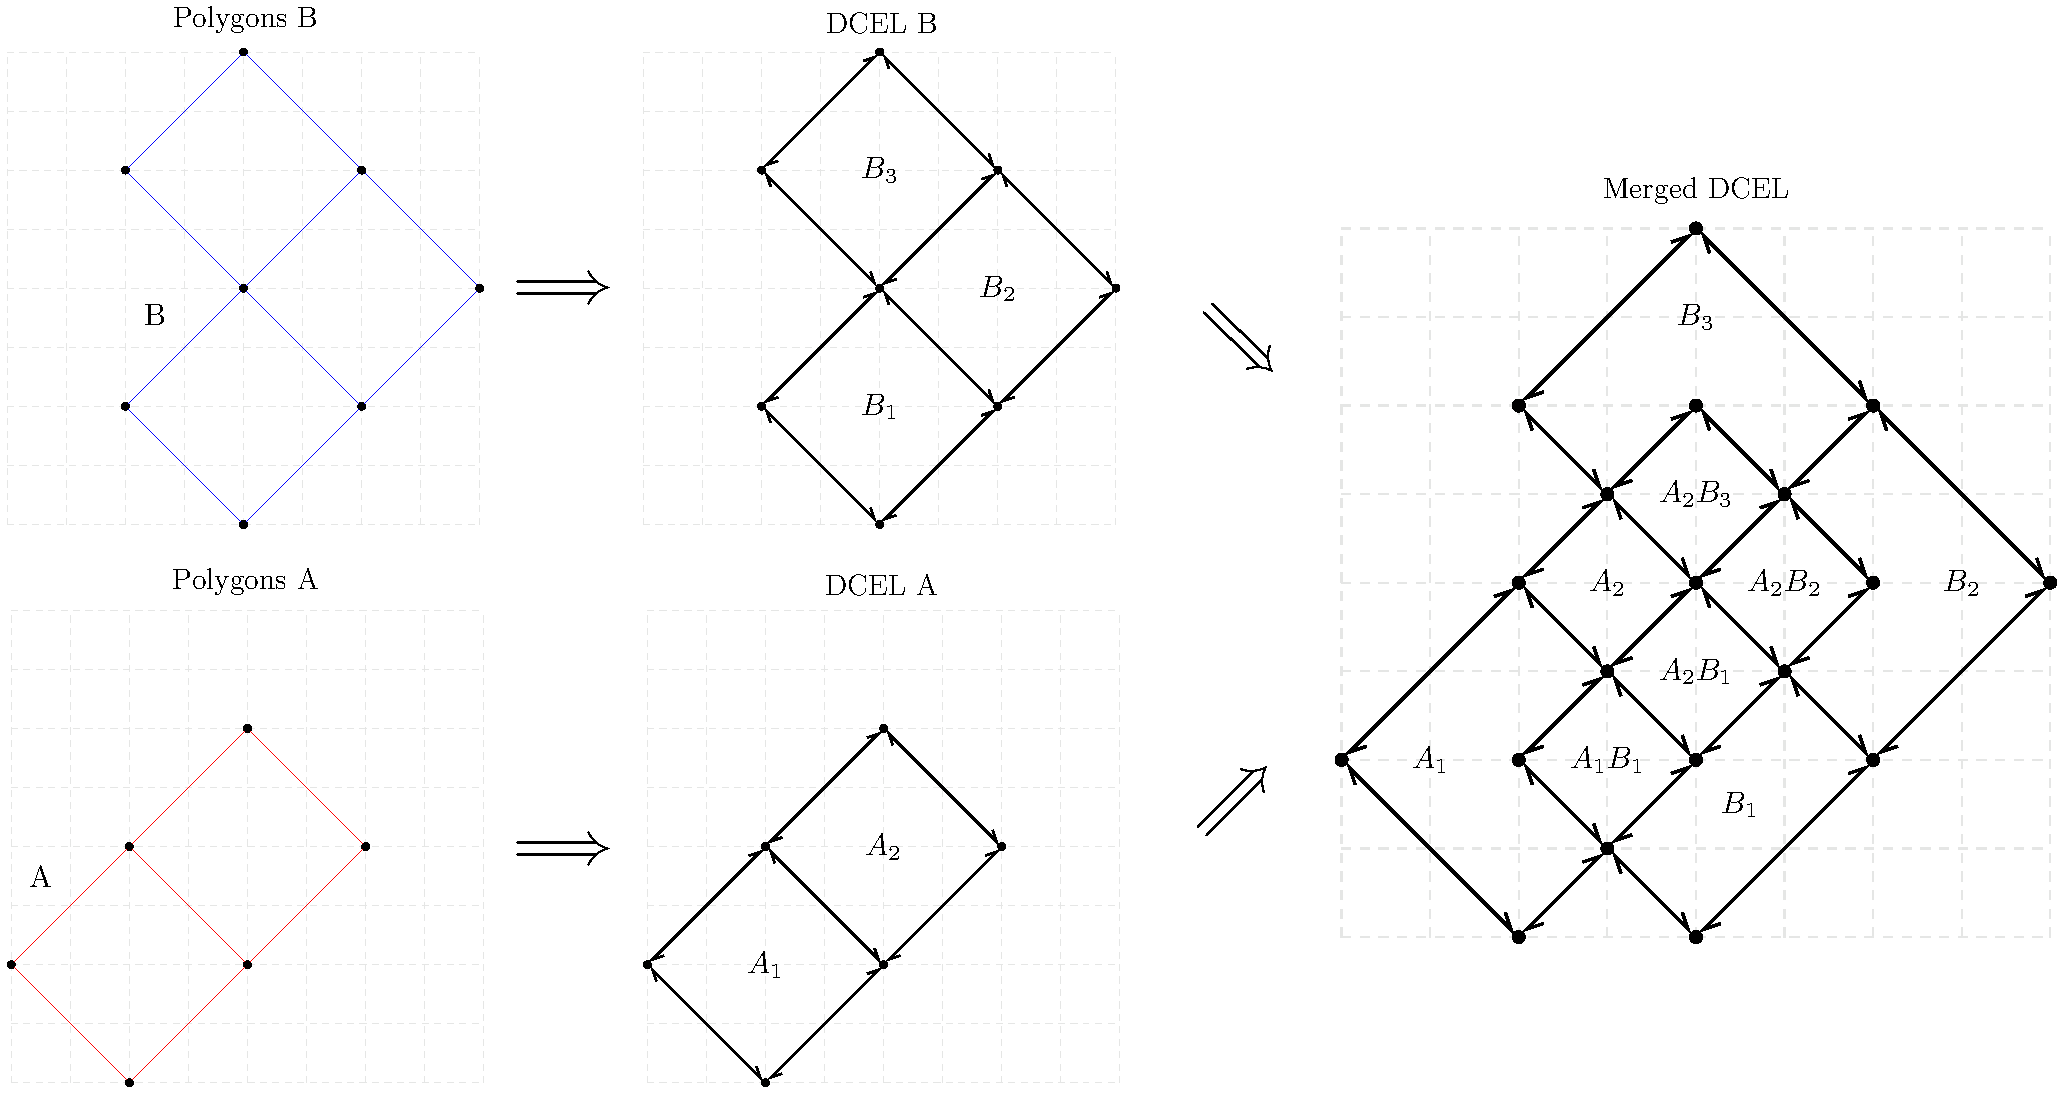
\includegraphics[width=\linewidth]{figures/SimpleDCEL} 
\end{frame}

\begin{frame}{DCEL operations}
    \centering 
    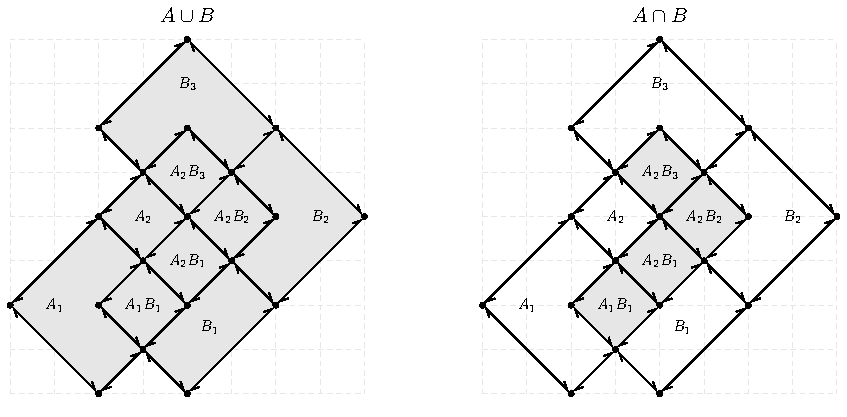
\includegraphics[width=0.8\linewidth]{figures/OverlayOperations1} 
\end{frame}

\begin{frame}{DCEL operations}
    \centering 
    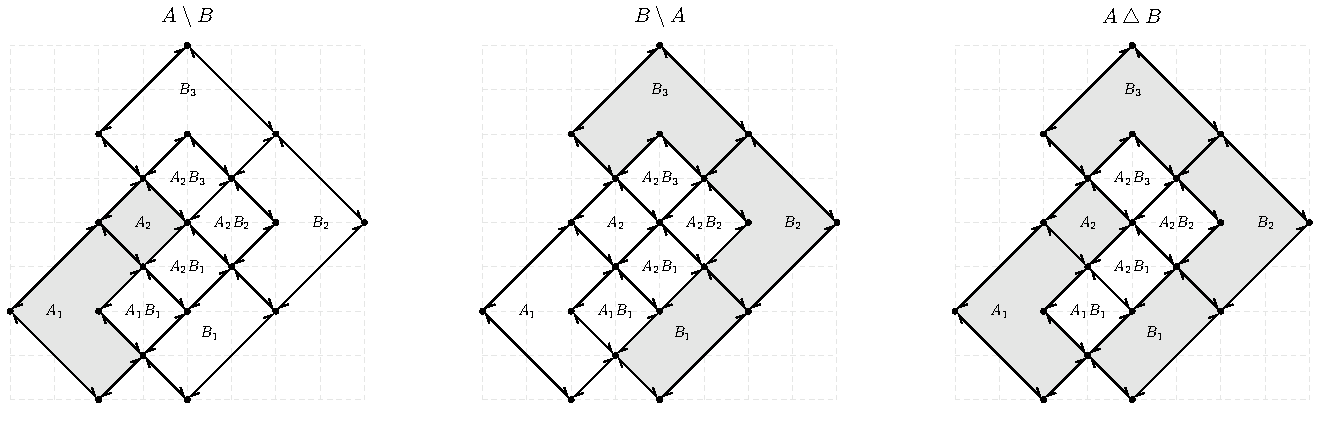
\includegraphics[width=\linewidth]{figures/OverlayOperations2} 
\end{frame}

\begin{frame}{Parallel DCEL construction}
    \centering 
    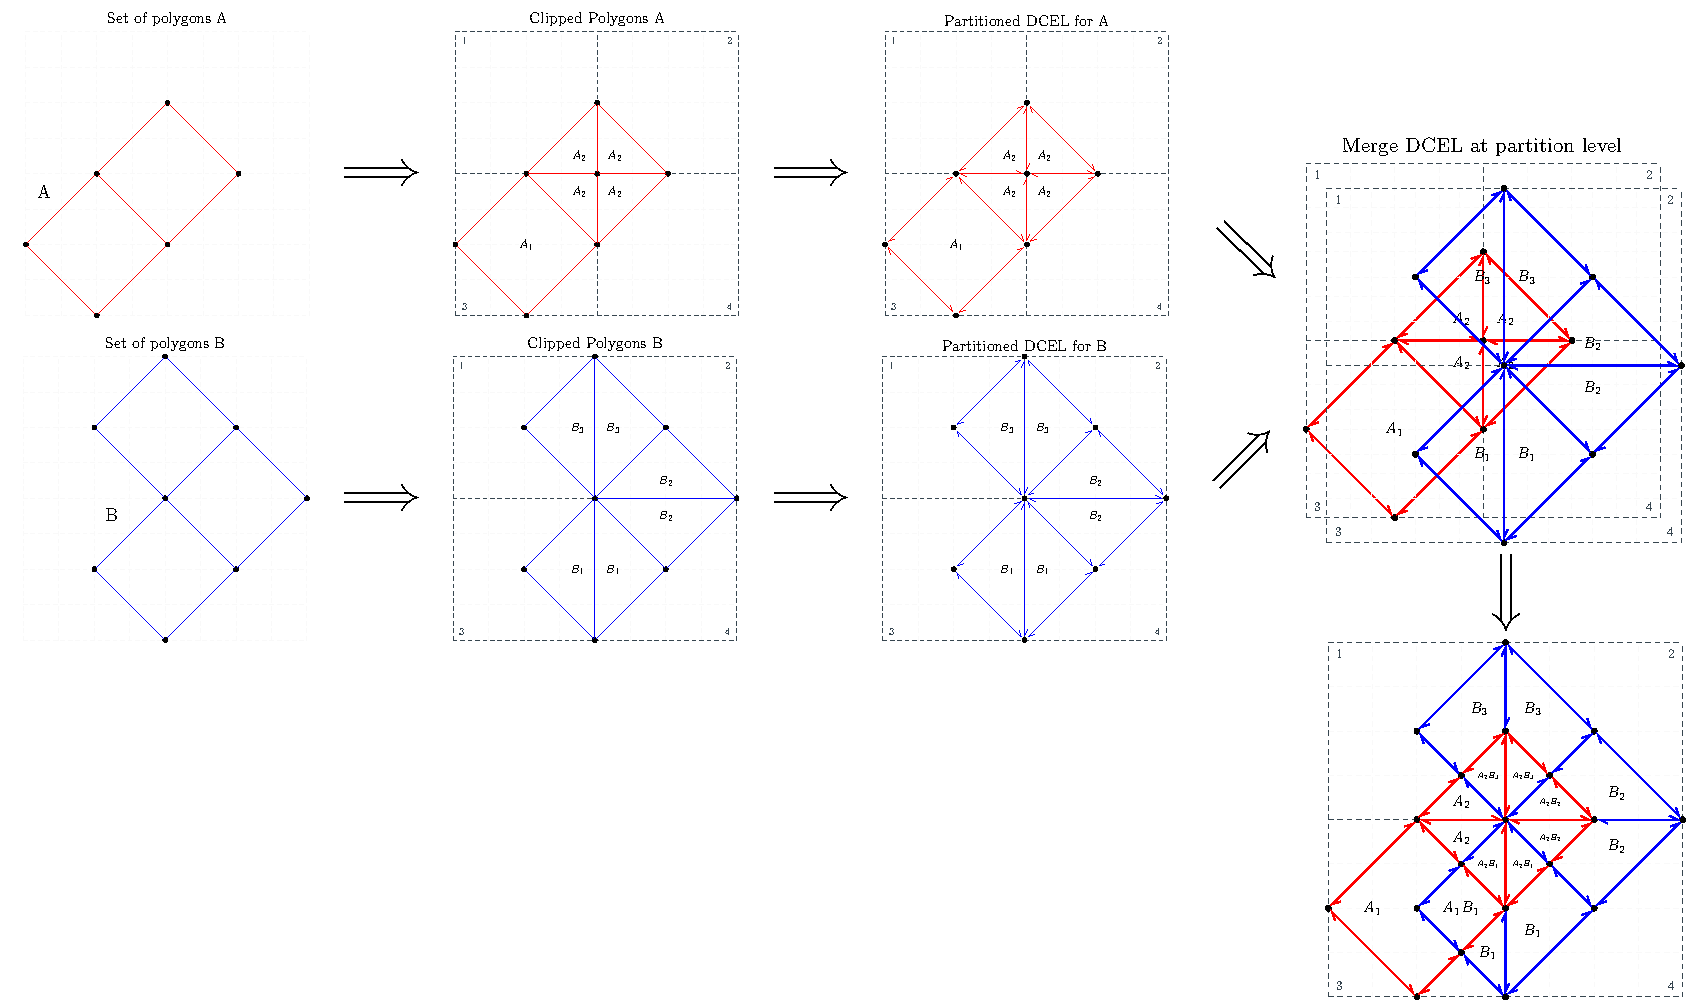
\includegraphics[width=\linewidth]{figures/OverlayParted1} 
\end{frame}

\begin{frame}{Parallel DCEL operations}
    \centering 
    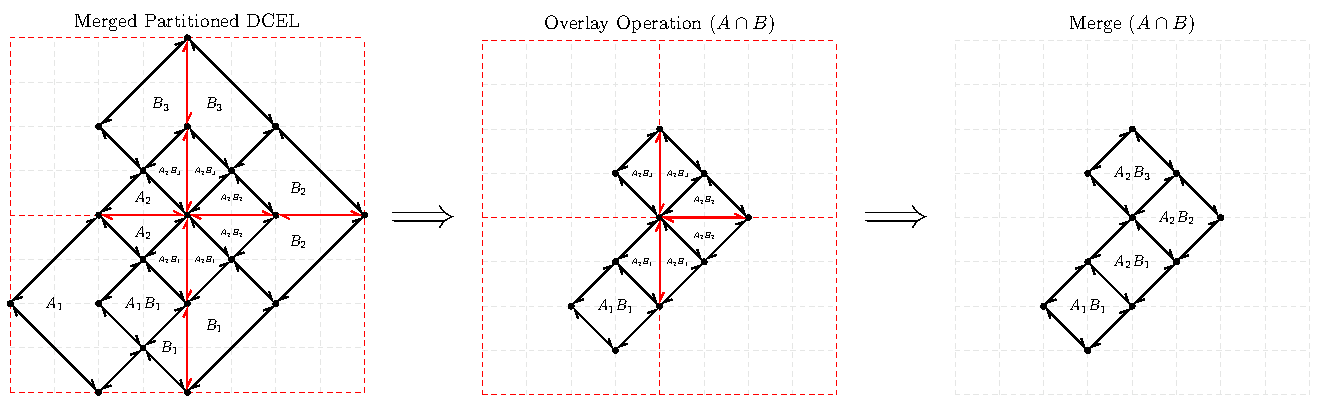
\includegraphics[width=\linewidth]{figures/OverlayParted2} 
\end{frame}

\begin{frame}{What is next...}
    \begin{itemize}
        \item \textbf{Current state:} Merged Partitioned DCEL is done.
        \item Working on Overlay operations.
        \item Additional testing.
    \end{itemize}
\end{frame}

\begin{frame}{Phili dataset}
    \begin{itemize}
        \item Philadelphia counties 2010
        \item 385 polygons
    \end{itemize}

    \centering 
    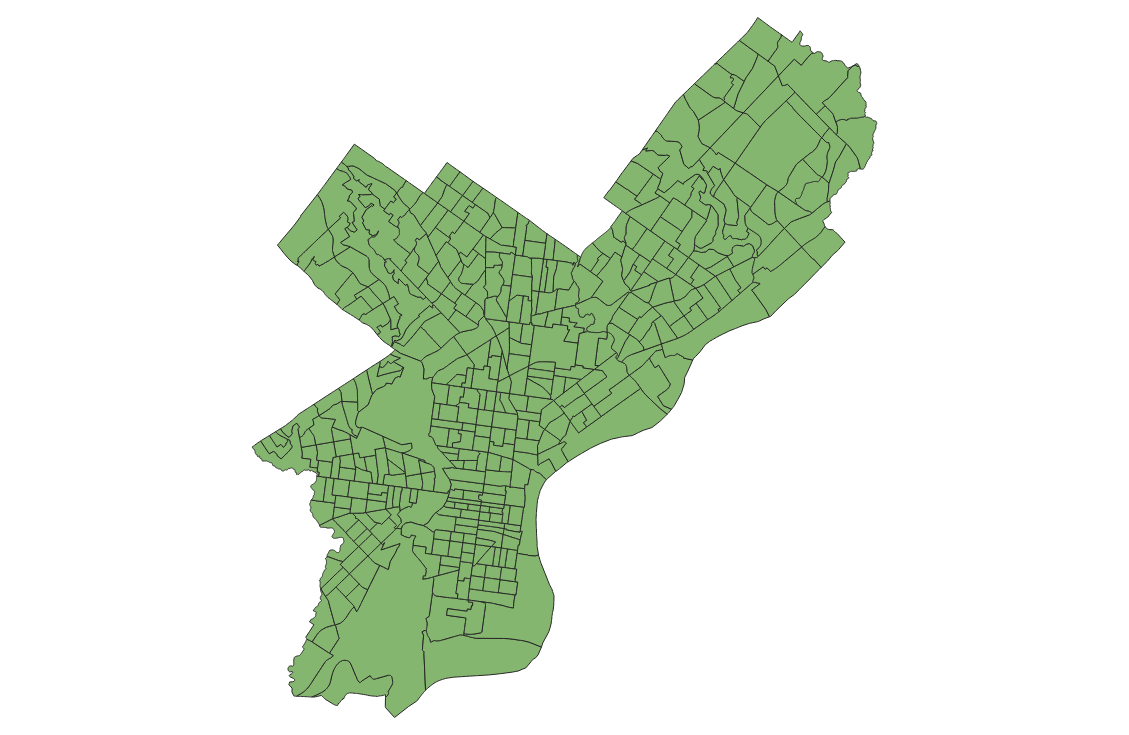
\includegraphics[width=0.8\linewidth]{figures/PhiliTest0.png} 
\end{frame}

\begin{frame}{Phili dataset}
    \centering 
    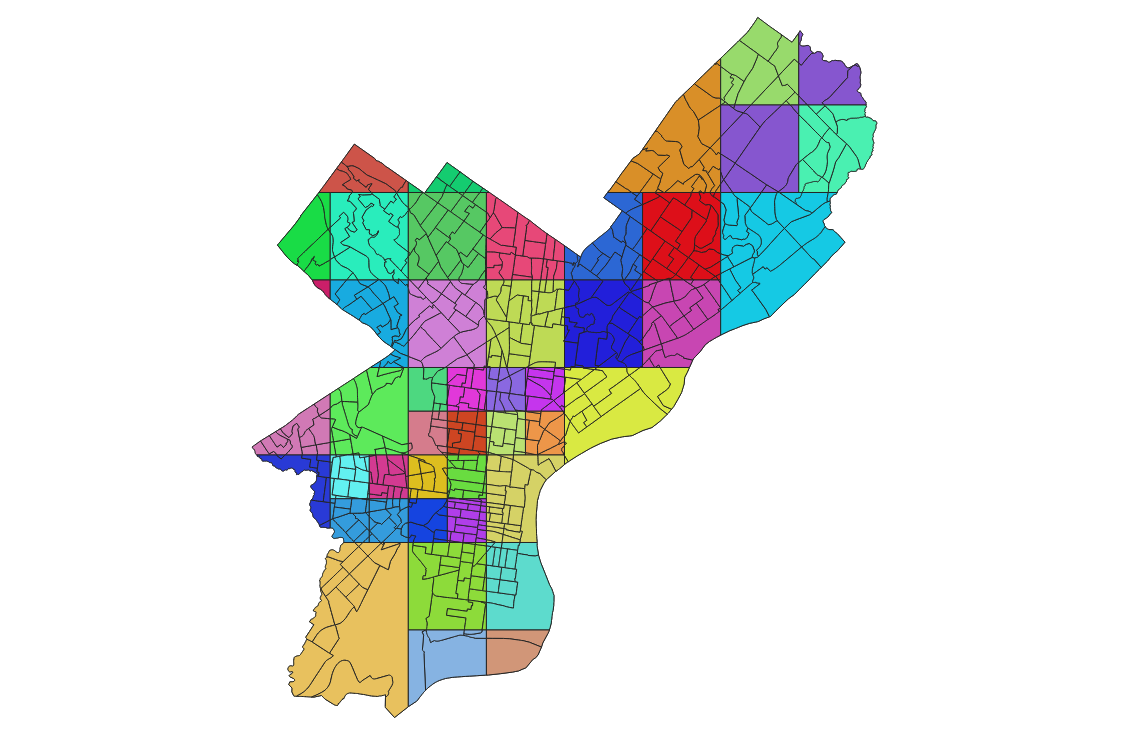
\includegraphics[width=0.8\linewidth]{figures/PhiliTest1.png} 
\end{frame}

\begin{frame}{Phili dataset}
    \centering 
    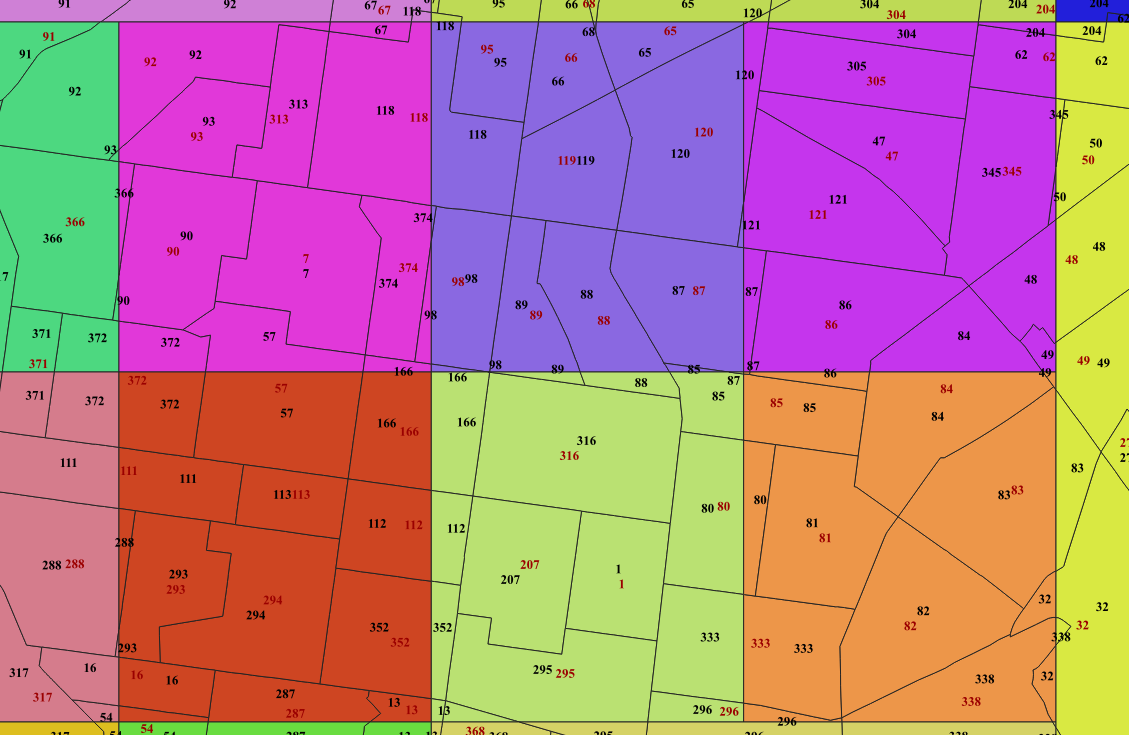
\includegraphics[width=0.9\linewidth]{figures/PhiliTest2.png} 
\end{frame}

\begin{frame}{Phili dataset}
    \begin{itemize}
        \item $R^2 = 1.0$
        \item $RMSE = 0.0299\ (\approx3cm^2)$
    \end{itemize}
    \centering 
    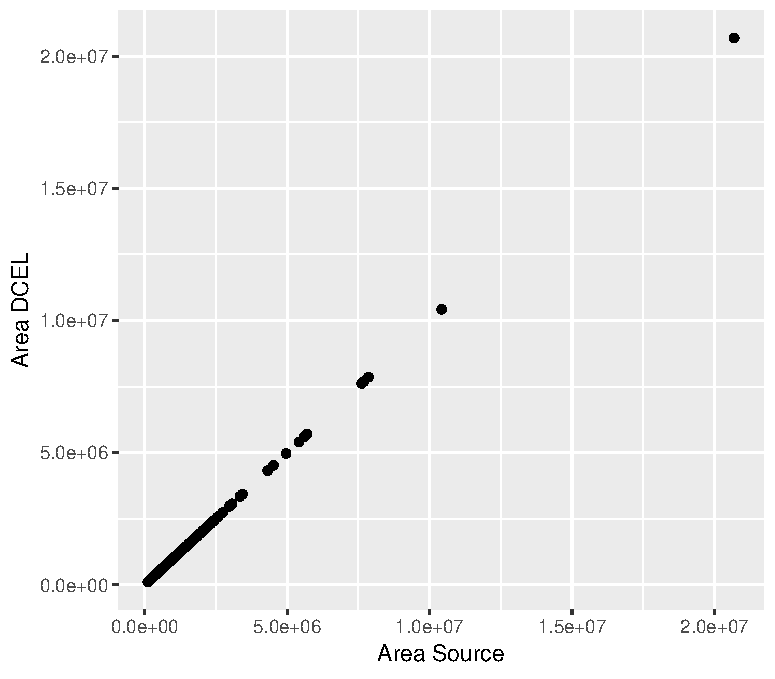
\includegraphics[width=0.55\linewidth]{figures/PhiliDiff} 
\end{frame}

\begin{frame}{Some notes}
    \begin{itemize}
        \item Some problems with larger dataset:
        \begin{itemize}
            \item How to deal with multipolygons and holes?
        \end{itemize}
    \end{itemize}
    \centering 
    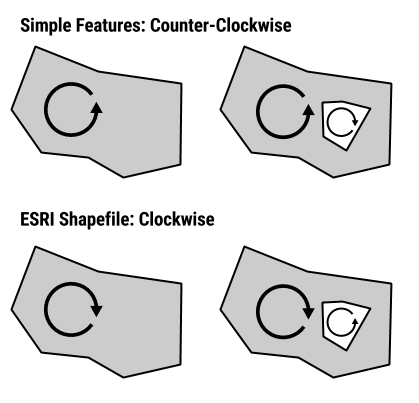
\includegraphics[width=0.4\linewidth]{figures/PolygonOrientation.png} 
\end{frame}

\end{document}
